\documentclass[11pt]{article}
\usepackage[margin=0.9in]{geometry}
\usepackage{amsmath,amssymb}
\usepackage{booktabs,enumitem,xcolor,array,tabularx,graphicx,float}
\usepackage{microtype}
\usepackage[most]{tcolorbox}
\usepackage[colorlinks=true,linkcolor=blue!50!black,urlcolor=blue!50!black]{hyperref}
\newcolumntype{Y}{>{\raggedright\arraybackslash}X}
\setlength{\parskip}{4pt}
\setlength{\parindent}{0pt}
\setlist{leftmargin=*,itemsep=1pt,topsep=2pt}
\newcommand{\E}{\mathbb{E}}
\graphicspath{{figures/}{../paper/figures/}}
\hypersetup{pdftitle={RLVR project brief: diagnosis and method}}
\newtcolorbox{idea}[1]{colback=blue!3,colframe=blue!40!black,fonttitle=\bfseries,title=#1,boxrule=0.6pt,arc=2pt}
\newtcolorbox{found}[1]{colback=green!3,colframe=green!40!black,fonttitle=\bfseries,title=#1,boxrule=0.6pt,arc=2pt}
\newtcolorbox{now}[1]{colback=orange!4,colframe=orange!60!black,fonttitle=\bfseries,title=#1,boxrule=0.6pt,arc=2pt}

\title{\textbf{Reward Shaping Is Noise Shaping}\\[4pt]\large A short brief: the idea, the diagnosis, the method, and where it stands}
\author{Mohamed Ayman\\\small October 21, 2026}
\date{}

\begin{document}
\maketitle
\vspace{-12pt}

\begin{idea}{The whole project in five sentences}
\begin{enumerate}
\item In RL with verifiable rewards (RLVR), many methods change how answers are scored (reward right ones, penalize wrong ones, change the baseline, aim at pass@$k$) and claim more \emph{diversity}.
\item They are compared at the same training step; a method that learns more slowly is less sharpened at that step, so it \emph{looks} more diverse.
\item We prove that every correctness-only scoring rule pushes the model the same way on average and differs only in noise; noise sets the \emph{speed} along one accuracy--diversity curve, not the curve.
\item Experiments on two model families confirm it, and adding noise alone recreates the effect of the best-known method (NSR).
\item Diversity at equal accuracy is only how evenly success is spread across questions, so a real method must bring new signal to rarely solved questions; we are now testing one that does.
\end{enumerate}
\end{idea}

\section{The words you need}
\begin{tabularx}{\linewidth}{@{}p{0.2\linewidth}Y@{}}
\toprule
pass@1 & Accuracy: the chance one sampled answer is right.\\
pass@$k$ & The chance at least one of $k$ answers is right: the usual measure of ``diversity'' or coverage.\\
Update & $g=\sum_i A_i\nabla\log\pi(y_i)$: each answer $y_i$ is pushed up or down by its advantage $A_i$.\\
Dr.\ GRPO & $A=r-\bar r$ (reward minus the group's mean); the standard, low-noise baseline.\\
PSR / NSR & Reward right answers only ($A=r$) / penalize wrong answers only ($A=r-1$). NSR is claimed to preserve diversity.\\
Matched accuracy & Compare pass@16 \emph{at the same pass@1}, by interpolating along the reference run's training curve.\\
\bottomrule
\end{tabularx}

\section{The theory}
For any rule that scores answers from their correctness, with $p$ a question's success rate:
\[\E g=c(p)\,\nabla p,\qquad \E\|g\|^2=F_1D_1(p)+F_0D_0(p)+\|\nabla p\|^2X(p),\]
where $F_1$ and $F_0$ are the mean squared gradients of a right and a wrong answer. The \emph{direction} is always $\nabla p$; a rule can only reweight questions ($c(p)$) and change the noise ($D_1, D_0$). PSR and NSR have the same mean; NSR is PSR plus zero-mean noise, carried by the wrong answers, which have 2--3$\times$ larger squared gradients (measured on both families).

\textbf{A useful identity.} At matched pass@1, pass@$k=\E_x[1-(1-p_x)^k]$ is concave in each question's $p_x$, so it is highest when success is spread evenly across questions. Diversity at equal accuracy measures that spread, nothing else.

\section{The diagnosis (finished)}
\begin{found}{Four findings}
\begin{enumerate}
\item \textbf{One curve.} On Qwen2.5-Math-1.5B, PSR, NSR, five baselines in between, the NSR paper's own implementation and a pass@4 objective all move along one accuracy--diversity curve. On OLMo-2-1B: NSR minus PSR at matched accuracy $-0.30$, 90\% [$-1.28$, $+0.77$], \textbf{equivalent within $\pm2$}; NSR is 19--22$\times$ noisier.
\item \textbf{Noise is the cause.} Adding to PSR a random-sign term of NSR's size (same mean) makes it exactly as slow as NSR: speed $\phi=-0.11$ [$-0.22$, $-0.05$] on a scale where NSR $=0$ and PSR $=1$. NSR at twice the learning rate recovers its lag. All stay on one curve (3 fresh seeds).
\item \textbf{The theory's noise formula fits} training within 0.69--1.18 once gradient sizes are re-measured; the right/wrong asymmetry fades from about 3$\times$ to 1.5$\times$ during training. With Adam, noise does not shrink steps; it misdirects them (13--27\% less aligned).
\item \textbf{Not a temperature effect.} RL barely changes entropy on fixed text (1.081 $\to$ 1.064) but cuts it 3--4$\times$ on its own samples: it steers into confident paths. Sampling a late checkpoint hotter does not beat the training curve ($-1.42$, 90\% [$-2.19$, $-0.68$], 511 problems).
\end{enumerate}
\end{found}

\begin{figure}[H]
\centering
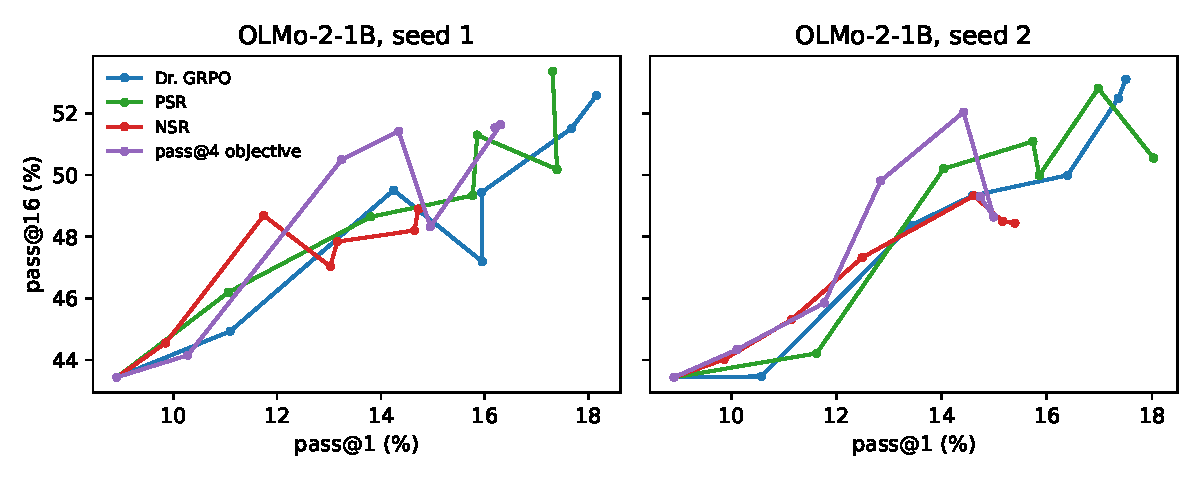
\includegraphics[width=0.49\linewidth]{olmo_curves.pdf}\hfill
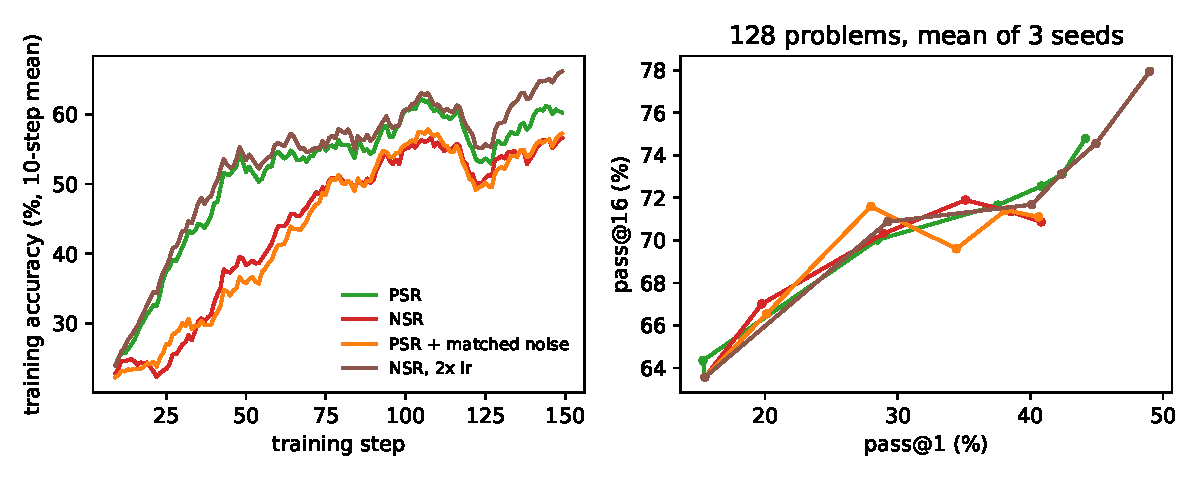
\includegraphics[width=0.49\linewidth]{noise_test.pdf}
\caption{Left: OLMo, five rules on one accuracy--diversity curve. Right: PSR plus matched noise (orange) learns as slowly as NSR (red); all lie on one curve.}
\end{figure}

\textbf{Independent review} (Codex as an ICML reviewer): 4/10 at first (claims too broad, cause not shown) $\to$ 5/10 after the noise test $\to$ \textbf{6/10} after the OLMo replication. To reach 7/10 the paper needs a method, derived from the diagnosis, that moves the curve.

\section{What the diagnosis says a method must do}
\begin{tabularx}{\linewidth}{@{}p{0.47\linewidth}Y@{}}
\toprule
Finding & Requirement\\
\midrule
Correctness-only rules share one curve & Bring information the current samples do not contain\\
Diversity $=$ spread of success across questions & Raise success on rarely solved questions\\
On those questions a group of 8 answers is usually all wrong & Supply signal exactly there\\
No global sharpening; entropy control blocks learning & Do not regulate entropy\\
Extra noise slows learning & Keep Dr.\ GRPO's low-noise update as the base\\
\bottomrule
\end{tabularx}

\section{Method, version 1: coverage-weighted memory (Pre-reg.\ 12)}
\begin{idea}{Coverage-weighted memory (CM)}
Train with Dr.\ GRPO. Store the verified, completed correct answers the model finds (at most 4 per question). Each step, replay 8 stored questions with an extra gradient $\lambda\nabla\log\sum_{y\in S_q}\pi(y\mid q)$, choosing questions in proportion to $k\,p(1-p)^{k-1}$ ($k=16$). That weight is exactly $\partial\,\mathrm{pass@}k/\partial\log p$: replay goes to questions solved about once in $k$, whose pass@$k$ can still rise.
\end{idea}

\textbf{Pilot} (1 seed, 255 validation problems): memory was the only family that lifted the curve (coverage memory $+2.1$; uniform memory $+0.2$); entropy bonus and the unlikeliness reward did nothing; entropy floors and adaptive entropy collapsed learning.

\textbf{Main runs} (3 fresh seeds, 511 test problems with audited answer keys). Pre-registered rule: \emph{moves the curve} if at least $+2$ points of pass@16 above Dr.\ GRPO's curve, including its best temperature, with the 95\% interval above 0, in all three seeds. Seeds 9 and 10 are complete; seed 8 waits for one evaluation.

\begin{center}\small
\resizebox{\linewidth}{!}{\begin{tabular}{@{}lccc@{}}
\toprule
Arm (seeds 9 and 10) & Gain at matched accuracy & 95\% interval & Step-150 pass@1 / greedy test acc.\\
\midrule
Dr.\ GRPO (reference) & 0 & & 44.3 / 48.1\\
\textbf{Coverage memory} & \textbf{$+1.0$} (seed 9: $+1.4$, seed 10: $+0.6$) & [$+0.3$, $+1.6$] & 42.5 / 48.0\\
Uniform memory & $+0.6$ & [$-0.1$, $+1.2$] & 42.9 / 47.4\\
Unlikeliness reward (published) & $+0.3$ & [$-0.4$, $+0.8$] & 43.5 / 47.5\\
\bottomrule
\end{tabular}}
\end{center}
\textbf{Reading.} A real lift, but half the $+2$ bar; the likely verdict is ``average agreement'' (within $\pm2$). Test accuracy is kept; sampled pass@1 is about 1.8 points lower. \textbf{Why so small:} in 150 steps each training question is visited about once; a group of 8 finds a success on a question with $p=1/16$ only 40\% of the time ($p=1/32$: 22\%), so the memory misses most of the questions it is meant to help.

\section{Method, version 2: seed the memory from the base model (Pre-reg.\ 14, running)}
Before training, sample the base model 32 times on every training question (``discovery''); this finds a success on a $p=1/16$ question 87\% of the time (for $p=1/32$: 64\%). Seed the memory with one base success per question; replace it once the model finds its own. Each arm answers one question about \emph{why} it works:

\begin{center}\small
\begin{tabularx}{\linewidth}{@{}p{0.32\linewidth}Y@{}}
\toprule
Arm (3 seeds each) & Question it answers\\
\midrule
\textbf{D32: seeded coverage memory} (candidate) & Does the method move the curve?\\
U32: seeded, uniform replay & Does the coverage weighting matter?\\
S32: fine-tune on the same successes, then plain RL & Does continual replay beat a one-off warm start?\\
C05: unseeded coverage memory, same strength & Does the seeding matter?\\
G32: plain Dr.\ GRPO, groups of 32 & Is it just ``more samples''?\\
\bottomrule
\end{tabularx}
\end{center}

\textbf{Pre-registered win:} D32 at least $+2$ points above Dr.\ GRPO's curve and temperature envelope (95\% interval above 0, all three seeds) \emph{and} equal final accuracy (90\% interval within $\pm1$); each mechanism claim needs D32 $\ge+1$ over that arm's curve. All six tests are corrected together (Holm). Declared and reviewed by Codex before any training; amendments recorded before outcomes.

\begin{now}{{Status on October 21, 2026}}
\begin{itemize}
\item Smoke test passed: all arms run, the memory is seeded with 3,904 questions, base traces retire as the model finds its own successes, memory use equals Dr.\ GRPO's.
\item Discovery: 6 of 8 shards done; the last two wait for GPUs (capacity is scarce in all three regions).
\item G32 training started (seed 9 running, seeds 8 and 10 queued). The other four arms start when discovery finishes: about 3.5 h of training, then about 4 h of evaluation.
\end{itemize}
\end{now}

\section{What each outcome means for the paper}
\begin{tabularx}{\linewidth}{@{}p{0.3\linewidth}Y@{}}
\toprule
Outcome & Paper\\
\midrule
D32 wins, and beats U32, S32, G32 & Diagnosis $+$ a method derived from it (the 7/10 target); next, replicate on OLMo.\\
D32 wins but ties a control & The method works; the mechanism claim is scoped (e.g.\ ``more samples help'').\\
No win & A strong diagnostic paper: popular diversity fixes (NSR, entropy control, unlikeliness, pass@$k$ objectives) do not move the curve, the theory says why, and replay of rare successes is the only lever that moved it (about 6/10).\\
\bottomrule
\end{tabularx}

\vspace{4pt}
\small Every experiment was pre-registered and reviewed before launch; the full story, with all twelve experiments, is in \texttt{report/story.pdf}.
\end{document}
